\documentclass[12pt]{fphw}

\usepackage[utf8]{inputenc}
\usepackage[T1]{fontenc}
\usepackage{mathpazo}
\usepackage{alphabeta}
\usepackage{graphicx}
\usepackage{booktabs}
\usepackage{listings}
\usepackage{enumerate}
\usepackage{hyperref}
\usepackage{amsmath}
\usepackage{framed}
\usepackage[framed]{ntheorem}
\usepackage{amssymb}
\usepackage{xcolor}
\usepackage{tabularx}
\usepackage{tikz}
\usepackage{float}
\usepackage{array}

\graphicspath{{./figures/}}

\setlength{\parskip}{\baselineskip}

\newframedtheorem{frm-thm}{Theorem}
\hypersetup{
    colorlinks=true,
    linkcolor=blue,
    filecolor=magenta,
    urlcolor=cyan,
}
\urlstyle{same}

\title{Deep Learning for NLP -- Homework 2 \\ Response Clarity Classification (CLARITY)}
\author{Αλέξανδρος Γκιάφης \\ ID: sdi2200284}
\date{Spring Semester 2025-2026}
\institute{National and Kapodistrian University of Athens \\ Department of Informatics and Telecommunications}
\class{Artificial Intelligence II (YS19 Μ226 Μ262 Μ325 Μ405)}

\begin{document}
\maketitle

{
  \hypersetup{linkcolor=black}
  \tableofcontents
}
\newpage

\section{Abstract}

Σε αυτή την εργασία είχαμε ένα dataset (το CLARITY) με ζευγάρια ερώτηση--απάντηση από πολιτικούς και έπρεπε να φτιάξουμε ένα μοντέλο που, για κάθε ζευγάρι, θα προβλέπει σε ποια από τις τρεις κατηγορίες ανήκει η απάντηση: \emph{Clear Reply} (ο πολιτικός όντως απαντάει), \emph{Clear Non-Reply} (ξεφεύγει εντελώς), ή \emph{Ambivalent} (η απάντηση είναι κάπου στη μέση -- λέει κάτι αλλά υπεκφεύγει κιόλας). Στην πρώτη εργασία είχα χρησιμοποιήσει κλασικές μεθόδους τύπου TF-IDF + Logistic Regression. Εδώ έπρεπε να γυρίσω σε deep learning και συγκεκριμένα σε Transformer-based μοντέλα.

Ξεκίνησα σταδιακά: πρώτα DistilBERT \cite{sanh2019distilbert} γιατί είναι το πιο ελαφρύ και πρόλαβα να κάνω πολλά πειράματα γρήγορα, μετά BERT \cite{devlin2019bert} σαν standard reference, και τέλος DeBERTa-v3-base \cite{he2021deberta} που είναι το πιο δυνατό από τα τρία και ήταν ο τελικός μου ``πρωταγωνιστής''. Πάνω στο DeBERTa πειραματίστηκα με αρκετά τρικ -- άλλα δούλεψαν, αρκετά όχι, και νομίζω ότι από τις αποτυχίες έμαθα περισσότερα από ό,τι από τις επιτυχίες.

Το καλύτερο public Kaggle αποτέλεσμα ήταν 0.69 macro-F1, που με έβγαλε γύρω στην 31η θέση στο public leaderboard. Στο τοπικό μου validation set, το καλύτερο score έφτασε 0.7136 macro-F1, με ensemble τριών διαφορετικών εκδοχών του ίδιου DeBERTa μοντέλου. Το ότι το Kaggle πέφτει λίγο σε σχέση με το local val είναι αναμενόμενο -- δεν είναι ακριβώς ίδιο data distribution, οπότε αυτό μου έδωσε και μια ρεαλιστική ιδέα του πόσο γενικεύει το μοντέλο μου.

\section{Εισαγωγή στο task και τι είχα να κάνω}

\subsection{Τι είναι το πρόβλημα}

Το CLARITY task ακούγεται απλό αλλά δεν είναι. Φαντάσου ότι ένας δημοσιογράφος ρωτάει έναν πρόεδρο: \emph{``Why are you not having a joint press conference with Putin?''}. Ο πρόεδρος μπορεί:

\begin{itemize}
    \item να απαντήσει ευθέως (\emph{Clear Reply}),
    \item να αλλάξει εντελώς θέμα (\emph{Clear Non-Reply}),
    \item ή -- και αυτό είναι το συχνότερο -- να πει κάτι που φαίνεται απάντηση αλλά στην ουσία είναι μισή ή ξεγλιστράει (\emph{Ambivalent}).
\end{itemize}

Το δύσκολο είναι ότι οι πολιτικές απαντήσεις σπάνια είναι ή τελείως clear ή τελείως evasion. Συχνά ένας πολιτικός θα πει 5 προτάσεις γενικότητες και μετά μία πρόταση που πραγματικά απαντάει, ή θα δώσει context και αιτιολογήσεις και μετά θα ``ξεχάσει'' να καταλήξει. Η Ambivalent κατηγορία είναι ουσιαστικά η ``γκρίζα ζώνη''. Αυτό σημαίνει ότι το μοντέλο δεν μπορεί απλώς να ψάξει keywords. Πρέπει να καταλάβει αν η απάντηση όντως απαντάει στην \textit{ερώτηση} -- δηλαδή πρέπει να συνδέσει το semantic content της απάντησης με αυτό που ζητήθηκε.

\subsection{Τι έπρεπε να φτιάξω, σύμφωνα με το assignment}

Σύμφωνα με τις οδηγίες του Homework 2, έπρεπε:

\begin{enumerate}
    \item να κάνω fine-tuning σε τρία συγκεκριμένα pretrained Transformer μοντέλα: \texttt{bert-base-uncased}, \texttt{distilbert-base-uncased}, και \texttt{microsoft/deberta-v3-base},
    \item να γράψω δικό μου training loop σε PyTorch (απαγορευόταν το Hugging Face \texttt{Trainer} API),
    \item να αποφασίσω εγώ πώς θα φτιάξω το input, πόσα epochs, ποιον optimizer, learning rate, max length κ.λπ.,
    \item να συγκρίνω τα τρία μοντέλα μεταξύ τους, να αναλύσω τα λάθη τους, και να δω αν διαφορετικά μεγέθη μοντέλων αποτυγχάνουν με διαφορετικό τρόπο,
    \item να υποβάλω 3 ξεχωριστά Kaggle notebooks (ένα ανά μοντέλο),
    \item να γράψω αυτό το report.
\end{enumerate}

\subsection{Τι είναι τέλος πάντων ένα Transformer (για να μη μένουν εκκρεμότητες)}

Πριν προχωρήσω στα πειράματα νομίζω ότι αξίζει να κάνω μια σύντομη εξήγηση των βασικών εννοιών, γιατί μετά αναφέρομαι σε αυτές συνέχεια. Αν ο αναγνώστης τα ξέρει ήδη, μπορεί να προσπεράσει.

Ένα \textbf{Transformer μοντέλο} είναι ένα νευρωνικό δίκτυο που επεξεργάζεται ακολουθίες (όπως κείμενα), και η βασική του ``μαγική'' δουλειά είναι ένα στρώμα που λέγεται \textbf{self-attention}. Με απλά λόγια, για κάθε λέξη στο κείμενο το μοντέλο υπολογίζει ``πόσο σχετική είναι κάθε άλλη λέξη με αυτή τη λέξη'', και χρησιμοποιεί αυτή την πληροφορία για να φτιάξει μια αναπαράσταση της λέξης που να εξαρτάται από το context. Αυτό είναι σημαντικό γιατί η ίδια λέξη μπορεί να σημαίνει διαφορετικά πράγματα ανάλογα με τι υπάρχει γύρω της (``bank'' σε bank account vs river bank).

\textbf{Pretrained} σημαίνει ότι το μοντέλο έχει ήδη εκπαιδευτεί σε τεράστιες ποσότητες κειμένου από το internet, με tasks σαν ``μάντεψε ποια λέξη λείπει''. Έτσι έχει μάθει general γλωσσικά patterns πριν δει καν το δικό μας dataset. \textbf{Fine-tuning} σημαίνει ότι παίρνουμε αυτό το έτοιμο μοντέλο, βάζουμε από πάνω ένα μικρό classifier (κάτι σαν τελικό linear layer που βγάζει 3 logits, ένα ανά κλάση), και συνεχίζουμε την εκπαίδευση στα δικά μας πιο λίγα δεδομένα. Έτσι ``προσαρμόζεται'' το μοντέλο στο specific task.

\textbf{Tokenizer}: τα Transformer δεν δουλεύουν με ολόκληρες λέξεις, τις κόβουν σε υπολέξεις (subwords) με βάση μια τεχνική σαν το BPE ή το SentencePiece. Παράδειγμα: η λέξη ``unhappiness'' μπορεί να γίνει [``un'', ``happi'', ``ness'']. Έτσι το μοντέλο δεν χάνεται όταν συναντάει λέξη που δεν έχει ξαναδεί -- την σπάει σε γνωστά κομμάτια.

\textbf{Embedding}: ένα διάνυσμα από αριθμούς που αναπαριστά μια λέξη ή ολόκληρο πρόταση. Π.χ. το \texttt{[CLS]} token (ένα ειδικό token που μπαίνει στην αρχή κάθε input στο BERT) μετά το pass από το μοντέλο γίνεται ένα διάνυσμα 768 διαστάσεων που ``περιέχει'' περιεκτικά την πληροφορία όλης της πρότασης -- και πάνω σε αυτό βάζουμε τον classifier για να βγάλουμε τις 3 κλάσεις.

\section{Data processing and analysis}

\subsection{Pre-processing}

Το αρχικό training set είχε 3448 γραμμές. Έκανα ένα σχετικά συντηρητικό cleaning και έμειναν 3412 παραδείγματα. Συγκεκριμένα:

\begin{enumerate}
    \item \textbf{Αφαίρεση contradictory duplicates}: είχε μερικά ζευγάρια Q-A που εμφανίζονταν δύο ή περισσότερες φορές με \emph{διαφορετικό} label. Αυτό για το μοντέλο είναι θόρυβος -- το ίδιο input δεν μπορεί να έχει δύο διαφορετικά labels και να βγάζει νόημα. Τα έβγαλα.
    \item \textbf{Αφαίρεση κάποιων προβληματικών rows} που είχα εντοπίσει στην πρώτη εργασία (πολύ μικρό text, OOV-heavy κλπ).
\end{enumerate}

Το βασικό μου axiom από εκεί και πέρα ήταν: \emph{δεν κάνω heavy cleaning του φυσικού κειμένου}. Τα Transformer είναι ήδη pretrained σε huge ποσότητες ακατέργαστου text, οπότε δεν θέλουν -- και πιθανόν χάνουν -- αν αρχίσω να αφαιρώ punctuation, να lowercaseάρω επιθετικά, να βγάζω stopwords κ.λπ. Επιπλέον στο συγκεκριμένο task μικρά linguistic σημάδια όπως ``well, ...'', ``I think...'', ``let me be clear'' είναι \emph{ακριβώς} ο τύπος της πληροφορίας που ξεχωρίζει μια clear απάντηση από μια ambivalent. Αν τα έσβηνα, θα έσβηνα σήμα.

\subsubsection{Word normalization (πιο εκλεπτυσμένη ιδέα)}

Δοκίμασα όμως μια πιο στοχευμένη μορφή normalization, η οποία τελικά βοήθησε λίγο. Η ιδέα: σε αυτό το task δεν μας ενδιαφέρει αν ο πολιτικός είπε ``in 1981'' ή ``in 1979''. Ενδιαφέρει το ότι αναφέρθηκε σε χρονιά. Οπότε αντικατέστησα patterns σαν χρονιές, ποσά, ποσοστά, ημερομηνίες με πραγματικές αγγλικές λέξεις: \texttt{year}, \texttt{money}, \texttt{percent}, \texttt{date}.

Σημαντικό: \textbf{έβαλα κανονικές αγγλικές λέξεις, όχι τεχνητά tokens} όπως \texttt{[A\_YEAR]}. Η διαφορά είναι κρίσιμη: το DeBERTa ξέρει τι σημαίνει \texttt{year}, έχει δει τη λέξη χιλιάδες φορές στο pretraining. Αν όμως του βάλω \texttt{[A\_YEAR]} σαν νέο token, πρέπει να μάθει embedding γι' αυτό \emph{από την αρχή} με μόνο 3000 παραδείγματα. Είναι σαν να του βάζω hieroglyphs. Ξανασυναντάμε αυτή τη διάκριση παρακάτω.

\subsection{Τι είδα στα δεδομένα}

\subsubsection{Class imbalance}

Οι τρεις κλάσεις δεν είναι ισόποσες. Η Ambivalent είναι η μεγαλύτερη (περίπου 60\%), η Clear Reply είναι μεσαία (περίπου 30\%), και η Clear Non-Reply είναι η μικρότερη (μόλις περίπου 10\%). Αυτή η ανισορροπία επηρεάζει τη μετρική: αν δίναμε περισσότερο βάρος σε accuracy, θα φτιάχναμε ένα μοντέλο που λέει συνέχεια ``Ambivalent'' και θα είχε αξιοπρεπές score. Γι' αυτό το macro-F1 είναι η σωστή μετρική -- δίνει ίσο βάρος και στις τρεις κλάσεις.

\subsubsection{Η ``γκρίζα'' Ambivalent κλάση}

Από τα διαγράμματα και την ανάλυση που έκανα, η Ambivalent ήταν η πιο μπερδευτική κατηγορία. Μοιάζει σαν μαγνήτης -- όταν το μοντέλο έχει αμφιβολία αν μια απάντηση είναι Clear ή Non-Reply, την πετάει στο Ambivalent. Λογικό, αν το σκεφτείς: αν ένα μοντέλο δεν είναι σίγουρο για το ποιο extreme να επιλέξει, η ``μέση'' κατηγορία είναι ασφαλής choice από άποψη loss.

Αυτό φαίνεται καθαρά στο τελικό confusion matrix του καλύτερου DeBERTa+numfeat single μοντέλου:
\[
C = \begin{bmatrix}
69 & 34 & 2 \\
34 & 155 & 13 \\
1 & 9 & 25
\end{bmatrix}
\]
Οι γραμμές είναι το πραγματικό label (CR / AMB / CNR), οι στήλες είναι η πρόβλεψη. Διαβάζοντάς το:
\begin{itemize}
    \item Από 105 πραγματικά Clear Reply, 34 πήγαν λάθος ως Ambivalent.
    \item Από 35 πραγματικά Clear Non-Reply, 9 πήγαν λάθος ως Ambivalent.
    \item Πολύ λίγα ``ακραία'' λάθη: μόλις 2 CR ταξινομήθηκαν ως CNR και 1 CNR ως CR. Δηλαδή το μοντέλο σπάνια κάνει το ``φοβερό'' λάθος του να μπερδέψει εντελώς τις δύο extreme κατηγορίες. Τα λάθη είναι σχεδόν πάντα ``slip το ένα τικ'' -- από CR ή CNR στο γειτονικό Ambivalent.
\end{itemize}

\subsection{Train / validation split}

Χώρισα τα 3412 cleaned examples σε:
\begin{itemize}
    \item train: 3070 (90\%)
    \item validation: 342 (10\%)
\end{itemize}
με \textbf{stratification ως προς το label}. Stratification σημαίνει ότι, αντί να πετάξουμε τυχαία 10\% στο val και να ελπίζουμε ότι θα είναι ισορροπημένο, αναγκάζουμε το split να κρατάει την αναλογία των κλάσεων ίδια με το αρχικό set. Αυτό είναι ιδιαίτερα σημαντικό όταν έχουμε mικρή κλάση (Clear Non-Reply): ένα τυχαίο split θα μπορούσε εύκολα να κρατήσει μόλις 20 ή 50 παραδείγματα CNR στο val, και το macro-F1 θα ήταν πολύ θορυβώδες.

Δεν έκανα cross-validation. Αρχικά γιατί δεν είχα όρεξη να χορεύω 5x χρόνο εκπαίδευσης για κάθε πείραμα, και κυρίως γιατί στα Transformer η μεγαλύτερη πηγή variance δεν είναι το split αλλά το \textbf{seed} (το αρχικό αρχικοποιημένο classifier head + dropout randomness). Οπότε για important runs δοκίμασα μερικά διαφορετικά seeds (συνήθως 42, 0, 1) πάνω στο ίδιο fixed split. Αυτό δίνει πιο καθαρή εικόνα, γιατί κρατάει το split σταθερό σε όλα τα μοντέλα.

\subsection{Vectorization (πώς γίνεται κείμενο σε αριθμούς)}

\subsubsection{Παλιό style: TF-IDF}

Στην πρώτη εργασία είχα χρησιμοποιήσει TF-IDF: κάθε κείμενο γίνεται ένα τεράστιο sparse διάνυσμα όπου κάθε διάσταση αντιστοιχεί σε μία λέξη ή n-gram, και η τιμή είναι μια συνάρτηση του πόσο συχνά εμφανίζεται η λέξη στο κείμενο πολλαπλασιασμένη με ένα weight που πέφτει αν η λέξη είναι common σε όλο το corpus (inverse document frequency). Λειτουργεί ικανοποιητικά για baseline αλλά:
\begin{itemize}
    \item αγνοεί τη \emph{σειρά} των λέξεων (``δεν θα απαντήσω'' = ``απαντήσω δεν θα'' στο TF-IDF),
    \item δεν καταλαβαίνει συνώνυμα ή παραφράσεις,
    \item δεν ``δεν συγκρίνει'' απάντηση με ερώτηση -- κάθε ένα είναι ξεχωριστό bag of words.
\end{itemize}

\subsubsection{Νέο style: Transformer contextual embeddings}

Με τα Transformer η αναπαράσταση είναι ριζικά διαφορετική. Ο tokenizer σπάει το κείμενο σε subwords, το μοντέλο τα περνάει από πολλά layers self-attention, και βγαίνουν \emph{contextual} embeddings -- δηλαδή το διάνυσμα της λέξης ``clear'' στη φράση ``let me be clear'' δεν είναι το ίδιο με το ``a clear answer''. Αυτό αλλάζει το παιχνίδι, γιατί το μοντέλο μπορεί να καταλάβει discourse markers, hedging, irony κ.λπ.

\subsubsection{Πώς ταΐζω την ερώτηση και την απάντηση μαζί}

Το input δεν ήταν μόνο η απάντηση. Το βασικό μου σχήμα ήταν \textbf{two-segment input}, δηλαδή:
\begin{verbatim}
[CLS] question_text [SEP] answer_text [SEP]
\end{verbatim}
Αυτό είναι ο standard τρόπος να δώσεις ζευγάρι κειμένων σε ένα BERT-family μοντέλο. Το μοντέλο μαθαίνει token type IDs (0 για το πρώτο segment, 1 για το δεύτερο) ώστε να ξέρει ποιο είναι ποιο, και η self-attention μπορεί να ``κοιτάει'' και τα δύο μαζί για να φτιάξει το τελικό sentence embedding. Δοκίμασα και \texttt{concat\_sep} (απλό concatenation με \texttt{[SEP]}) στο DistilBERT -- για το DistilBERT τα δύο σχήματα έβγαζαν \emph{ίδιες} προβλέψεις γιατί το DistilBERT δεν έχει token\_type\_ids embedding (έχει αφαιρεθεί στο distillation). Στο BERT/DeBERTa το two\_segment είναι το natural choice και έμεινα σε αυτό.

\section{Τα μοντέλα που δοκίμασα -- σύντομος οδηγός}

Σε αυτό το section εξηγώ με δύο λόγια τι είναι το καθένα από τα τρία μοντέλα που χρησιμοποίησα. Νομίζω χρειάζεται γιατί δεν είναι όλα ισοδύναμα -- το καθένα έχει διαφορετική αρχιτεκτονική και διαφορετικά τρικ.

\subsection{BERT (\texttt{bert-base-uncased})}

Το αυθεντικό BERT \cite{devlin2019bert}. Είναι ένα Transformer encoder με 12 layers, hidden size 768 και 110M parameters. ``Uncased'' σημαίνει ότι το vocabulary του δεν διαχωρίζει κεφαλαία/μικρά -- το ``Hello'' και το ``hello'' γίνονται το ίδιο token. Pretrained με δύο tasks: Masked Language Modeling (μάντεψε σβησμένες λέξεις) και Next Sentence Prediction (αν δύο προτάσεις είναι διαδοχικές). Το βασικό feature που κληρονόμησαν όλα τα παρόμοια μοντέλα είναι το \emph{bidirectional} self-attention -- κάθε token κοιτάει και αριστερά και δεξιά μέσα στο sentence ταυτόχρονα, αντί να διαβάζει left-to-right όπως κάνουν τα GPT-style μοντέλα.

\subsection{DistilBERT (\texttt{distilbert-base-uncased})}

Το DistilBERT \cite{sanh2019distilbert} είναι μια ``μαθήτρια'' εκδοχή του BERT. Ο τρόπος που το έφτιαξαν λέγεται \textbf{knowledge distillation}: παίρνεις ένα μεγάλο pretrained μοντέλο (το ``teacher'', εδώ BERT) και εκπαιδεύεις ένα μικρότερο (το ``student'') όχι απλώς να μαντέψει τα labels, αλλά να μιμηθεί τις probabilities του teacher. Έτσι το student τα καταφέρνει με σχεδόν τη μισή ποσότητα παραμέτρων (66M, 6 layers αντί 12), τρέχει σχεδόν διπλάσια γρήγορα, και χάνει μόνο γύρω στο 3\% accuracy σε generic tasks.

Επιπλέον το DistilBERT αφαιρεί το NSP loss και τα token\_type\_ids embedding. Πρακτικό consequence: στο dataset μας το DistilBERT \emph{δεν} χρησιμοποιεί την πληροφορία ``ποιο segment είναι ερώτηση και ποιο απάντηση''. Όλα τα tokens είναι ίδιο segment από την οπτική του μοντέλου.

Επέλεξα το DistilBERT σαν το μικρότερο και πιο γρήγορο μοντέλο, για να κάνω fast iteration στα πειράματα -- αν μια ιδέα δεν δούλευε στο DistilBERT, σπάνια άξιζε να σπαταλήσω χρόνο σε BERT/DeBERTa.

\subsection{DeBERTa-v3-base (\texttt{microsoft/deberta-v3-base})}

Το DeBERTa \cite{he2021deberta} -- ή πληρέστερα ``Decoding-enhanced BERT with disentangled Attention'' -- είναι σαν BERT αλλά κάνει δύο σημαντικά πράγματα διαφορετικά:

\begin{enumerate}
    \item \textbf{Disentangled attention.} Στο BERT, το embedding κάθε λέξης είναι (γενικά) embedding του ID της λέξης + positional embedding (πληροφορία θέσης), και αυτό το mash είναι που μπαίνει στη self-attention. Στο DeBERTa, η self-attention υπολογίζει ξεχωριστά το ``content-to-content attention'' και το ``content-to-position attention''. Με απλά λόγια: ο Pearson μάθαινε ένα ενιαίο διάνυσμα (``τι λέει η λέξη + πού βρίσκεται''), ενώ το DeBERTa μάθει δύο κανάλια (``τι λέει η λέξη'' και ``πού βρίσκεται'') και τα συνδυάζει πιο έξυπνα. Αυτό βοηθάει σε tasks όπου η σχετική θέση στοιχείων μετράει.
    \item \textbf{Enhanced mask decoder.} Στο pretraining, αντί να προβλέπει την σβησμένη λέξη μόνο από context, χρησιμοποιεί επίσης absolute positional information. Δεν έχει direct συνέπεια στο fine-tuning αλλά δίνει καλύτερα pretrained weights.
\end{enumerate}

Ειδικά το \texttt{deberta-v3-base} χρησιμοποιεί ELECTRA-style pretraining objective (replaced token detection αντί masked language modeling), που έχει δειχτεί ότι είναι πιο sample-efficient. Παρότι έχει ίδιο μέγεθος με το BERT-base (~140M params εδώ), συνήθως νικάει το BERT καθαρά σε classification tasks. Αυτό το επιβεβαίωσα και εγώ: από 0.6417 macro-F1 (BERT) στο 0.6962 (DeBERTa single seed=42) -- αρκετά μεγάλο jump.

\textbf{Πρακτικό warning για το DeBERTa:} είναι numerically πιο fragile από το BERT. Η πρώτη φορά που το έτρεξα, το loss έβγαινε \texttt{NaN} ή το μοντέλο κατέρρεε προβλέποντας μόνο Ambivalent. Έπρεπε να καθορίσω συγκεκριμένη έκδοση \texttt{transformers==4.44.0}, να βάλω \texttt{eps=1e-6} στον optimizer και να δώσω \emph{differential learning rate} (το head με 10$\times$ μεγαλύτερο learning rate από το backbone). Αυτό το έμαθα την πιο επώδυνη ρότα -- δηλαδή τρέχοντας πολλά αποτυχημένα runs μέχρι να βρω το συνδυασμό. Το αναφέρω εδώ γιατί νομίζω είναι useful negative finding: το DeBERTa είναι καλύτερο μοντέλο αλλά δεν είναι ``plug and play''.

\section{Algorithms and Experiments}

\subsection{Συνολική στρατηγική}

Η βασική μου ιδέα για τα πειράματα ήταν: \emph{ξεκίνα από το πιο μικρό και απλό, σιγά σιγά πήγαινε στο πιο μεγάλο και περίπλοκο, και σε κάθε βήμα κράτα baselines}. Η λογική είναι ότι αν ένα ``έξυπνο'' μοντέλο δεν κερδίζει το απλούστερο baseline, τότε κάτι πάει λάθος ή το trick που πρόσθεσα δεν αξίζει.

Άρα η πορεία ήταν:
\begin{enumerate}
    \item HW1 baseline (Logistic Regression + TF-IDF): 0.6017 macro-F1.
    \item DistilBERT vanilla: ανέβηκε σε ~0.64.
    \item BERT vanilla: παρόμοιο ~0.64.
    \item DeBERTa vanilla: jump στο ~0.69.
    \item DeBERTa + numeric side branch: best single 0.7007.
    \item DeBERTa ensembles διαφορετικών seeds και διαφορετικών views: best 0.7136 local val.
\end{enumerate}

\subsection{Πειράματα -- κύριος πίνακας}

\begin{table}[H]
\centering
\small
\begin{tabularx}{\textwidth}{lXrr}
\toprule
Trial & Περιγραφή & Val macro-F1 & Public Kaggle \\
\midrule
HW1 baseline & Logistic Regression + TF-IDF & 0.6017 & -- \\
DistilBERT & \texttt{max\_length=512}, lr $3 \cdot 10^{-5}$, 3 epochs, seed=42 & 0.6405 & -- \\
BERT & \texttt{max\_length=256}, lr $2 \cdot 10^{-5}$, 5 epochs, seed=1 & 0.6417 & -- \\
DeBERTa & two-segment, 3 epochs, seed=42, wd=0 & 0.6962 & ~0.68 \\
DeBERTa α-ensemble (3 seeds) & weighted avg over seeds 42/0/1 & 0.7070 & 0.68 \\
Feature tokens (failed) & handcrafted tags injected as text tokens & 0.6191 & -- \\
\textbf{DeBERTa + numeric side branch} & DeBERTa pooled vec + handcrafted feats via MLP & \textbf{0.7007} & \textbf{0.69} (31st) \\
More epochs (failed) & ίδια ιδέα με 6 epochs & 0.6876 & 0.67 \\
Rich features (failed) & πολλά extra HW1-style features & 0.6593 & 0.64 \\
Evasion stack (failed) & evasion-label probabilities ως extra features & 0.6503 & -- \\
Word normalization & αντικατάσταση αριθμών με κανονικές λέξεις & 0.6965 & -- \\
\textbf{Phase 18 alpha ensemble} & raw + wordnorm + focused view & \textbf{0.7136} & -- \\
Calibrated alpha & class multipliers post-hoc & 0.7154 & -- \\
Dual-view (failed) & shared DeBERTa σε full + focused & 0.6888 & -- \\
\bottomrule
\end{tabularx}
\caption{Συνολικός πίνακας πειραμάτων. Το final submitted Kaggle score είναι 0.69 (31η θέση).}
\label{tab:trials}
\end{table}

\subsection{Λεπτομέρειες ανά πείραμα -- τι δοκίμασα και τι έμαθα}

Εδώ θέλω να εξηγήσω αναλυτικά τι ακριβώς ήταν κάθε πείραμα, ειδικά αυτά που είχαν ``περίεργα'' ονόματα. Δεν θέλω να μένει αβέβαιο τι σημαίνει ``focused view'' ή ``dual-view'' ή ``evasion stack''.

\subsubsection{DistilBERT: ο φτηνός γρήγορος εξερευνητής}

Στο DistilBERT η σημαντικότερη ανακάλυψη ήταν ότι το \texttt{max\_length=512} βοηθούσε σαφώς. Όταν είχα \texttt{max\_length=128} ή \texttt{256}, πολλές μεγάλες πολιτικές απαντήσεις κόβονταν στη μέση -- και αυτό κατέστρεφε ακριβώς το σήμα που ήθελα. Με ml=512 όλη η απάντηση χωράει στο context. Best DistilBERT seed=42, lr 3e-5, 3 epochs, ml=512 = \textbf{0.6405} macro-F1.

Δοκίμασα επίσης πολλές μικρές παραλλαγές που \emph{δεν} βοήθησαν, και αναφέρω τις πιο interesting:

\begin{itemize}
    \item \textbf{Class weights στο cross-entropy loss}: ιδέα ήταν να δώσω μεγαλύτερο βάρος στα πιο σπάνια classes (CR, CNR) ώστε το μοντέλο να μην επικεντρώνεται μόνο στο Ambivalent. Αποτέλεσμα: 0.5955 (ίδιο config). Το CR βελτιώθηκε λίγο, το AMB έπεσε αρκετά, στο σύνολο macro-F1 χειρότερα.
    \item \textbf{Focal loss} ($\gamma=2.0$): ένα loss που down-weightάρει εύκολα παραδείγματα ώστε το μοντέλο να επικεντρώνεται στα δύσκολα. Έπεσε στο 0.6284 -- πιθανόν γιατί τα ``εύκολα'' ήταν ήδη το σωστό σήμα και το να τα αγνοεί δεν βοήθησε.
    \item \textbf{cw + focal συνδυασμός}: catastrophe, 0.4383. Το AMB κατέρρευσε από 0.78 σε 0.25 F1. Διπλή penalty στις κυρίαρχες κλάσεις -- το μοντέλο τρόμαξε να προβλέψει AMB.
    \item \textbf{Negation markers ([NEG] prefix στα verbs άρνησης}, με spaCy): πιο γλωσσολογικό trick, βάζω ένα marker πριν από κάθε verb σε άρνηση. Ιδέα: τα CNR συχνά έχουν αρνητικά verbs (``I won't say...''). +0.008 στο DistilBERT (0.6484 vs 0.6405). Μικρό improvement αλλά consistent.
    \item \textbf{Multi-task auxiliary head} (multi-task aux=0.3 με fixed 2-layer head): εδώ το dataset έχει ένα δευτερεύον label, το \texttt{evasion\_label} (πιο fine-grained, 9 κλάσεις: Explicit Reply, Claims Ignorance, Dodging, Clarification, ...). Multi-task σημαίνει ότι το μοντέλο εκπαιδεύεται σε ΔΥΟ tasks ταυτόχρονα: το main 3-class clarity \emph{και} το auxiliary 9-class evasion. Το σκεπτικό: τα δύο labels είναι σχετιζόμενα, οπότε ίσως η extra ``εργασία'' του να μάθει το λεπτομερές evasion να βοηθήσει τα clarity weights. Δούλεψε στο DistilBERT: \textbf{+0.020 mean} σε 3 seeds ($0.6367 \pm 0.012$ vs baseline $0.6167 \pm 0.021$). Επίσης \emph{μείωσε} το seed variance, που σημαίνει ότι λειτούργησε σαν regularizer.
\end{itemize}

\subsubsection{Από DistilBERT σε BERT: μικρή βελτίωση}

Όταν ports-άρα την winning DistilBERT config (ml=256, lr 2e-5, 5 epochs) στο BERT, είδα best 0.6417 (seed=1). Ουσιαστικά τα ίδια. Ενδιαφέρον finding: το multi-task aux που δούλεψε στο DistilBERT \emph{δεν} δούλεψε στο BERT -- ήταν πρακτικά tied με το baseline ($-0.002$). Παρόμοιο pattern και στο DeBERTa, όπου το aux \emph{έβλαψε} ($-0.049$).

Αυτό μου άρεσε σαν εύρημα: \textbf{auxiliary granularity helps weak representations αλλά βλάπτει strong ones}. Ένα DeBERTa έχει ήδη μάθει αυτές τις λεπτές διακρίσεις από το pretraining του -- δεν χρειάζεται extra βοήθεια, αντίθετα η extra task το ``μπερδεύει'' γιατί η evasion taxonomy σπάει την Ambivalent κλάση σε υποκατηγορίες που το DeBERTa είχε ήδη ομαδοποιήσει σωστά.

\subsubsection{DeBERTa baseline: το πραγματικό άλμα}

Το DeBERTa-v3-base seed=42 χωρίς κανένα trick -- απλά two-segment input, lr 2e-5, 3 epochs, ml=256, weight\_decay=0 -- έδωσε \textbf{0.6962} macro-F1. Αυτό είναι +0.05 πάνω από το BERT, ένα τεράστιο jump για NLP standards.

Φυσικά μόνο seed=42 δεν είναι αξιόπιστο. Έτρεξα και seeds 0 και 1 για να δω variance: 0.6333 (seed=0), 0.6727 (seed=1). Δηλαδή το seed=42 ήταν \textit{lucky}, αλλά ακόμα και ο μέσος όρος ($0.6674 \pm 0.032$) είναι σαφώς καλύτερος από το BERT/DistilBERT.

Με weighted ensemble των 3 seeds έφτασα 0.7070 local val και 0.68 στο Kaggle (39η θέση τότε).

\subsubsection{Ιδέα 1: Feature tokens μέσα στο κείμενο (απέτυχε)}

Από την HW1 είχα handcrafted features όπως: \texttt{HEDGE\_HIGH} (πολλά hedging words), \texttt{OV\_LOW} (λίγο overlap ερώτησης--απάντησης), \texttt{LEN\_HIGH} (μεγάλη απάντηση). Σκέφτηκα: ``ωραία, ας τα βάλω σαν ειδικά tokens μέσα στο input, ας πούμε στην αρχή της απάντησης. Έτσι το DeBERTa θα ``δει'' explicit signals''.

Δηλαδή το input γινόταν κάτι σαν:
\begin{verbatim}
[CLS] question [SEP] [HEDGE_HIGH] [OV_LOW] [LEN_HIGH] answer [SEP]
\end{verbatim}

Αποτέλεσμα: \textbf{0.6191}, πολύ κάτω από το vanilla DeBERTa (0.6962).

Γιατί απέτυχε; Γιατί αυτά τα tokens (\texttt{[HEDGE\_HIGH]} κ.λπ.) είναι \emph{καινούρια}, δεν υπάρχουν στο vocabulary του DeBERTa. Το μοντέλο πρέπει να μάθει embedding γι' αυτά \emph{από το μηδέν}, με μόλις 3000 παραδείγματα. Επιπλέον φέρονται σαν θόρυβος στην self-attention -- το DeBERTa δεν ξέρει αν είναι σημαντικά ή όχι. Στην πρώτη εργασία αυτά τα features δούλευαν επειδή ο linear classifier δεν είχε άλλη επιλογή -- χρησιμοποιούσε ό,τι του δίναμε explicit. Στο DeBERTa, η ίδια πληροφορία υπάρχει ήδη σιωπηρά μέσα στα contextual embeddings, και τα tokens απλώς βρωμίζουν τη ροή.

\textbf{Lesson learned}: το feature engineering της πρώτης εργασίας \emph{δεν} γίνεται transferred ως text tokens.

\subsubsection{Ιδέα 2: Numeric side branch (το breakthrough)}

Ίδια ιδέα, σωστή υλοποίηση. Αντί να μπω στα tokens, έφτιαξα τα features σαν \emph{αριθμητικό} input και τα έδωσα σε ξεχωριστό κανάλι. Αρχιτεκτονικά:

\begin{enumerate}
    \item Το DeBERTa διαβάζει κανονικά το two-segment input και βγάζει το pooled vector (768 dims).
    \item Παράλληλα, υπολογίζω 19 αριθμητικά features από το ζευγάρι Q-A: μήκος απάντησης (tokens, words, sentences), overlap ερώτησης--απάντησης, hedge density, negation count, evidence markers, κ.λπ.
    \item Τα features κανονικοποιούνται με statistics \emph{μόνο από το train split} (πολύ σημαντικό -- αν χρησιμοποιούσα και το val ή το test, θα είχα leakage).
    \item Περνάνε από ένα μικρό MLP (Linear $\rightarrow$ ReLU $\rightarrow$ Dropout $\rightarrow$ Linear) που τα μετατρέπει σε ένα 64-dim dense vector.
    \item Concat του DeBERTa pooled vector με το feature vector $\rightarrow$ τελικό classifier $\rightarrow$ 3 logits.
\end{enumerate}

Δηλαδή το DeBERTa βλέπει το text όπως πάντα, ``καθαρό'', και τα handcrafted features μπαίνουν με ένα παράλληλο, completely separate pathway που πάει κατευθείαν στον τελικό classifier. Δεν παρενοχλούν την self-attention.

Αποτέλεσμα: \textbf{0.7007} (seed=42, single model). +0.005 πάνω από το vanilla DeBERTa, και κρίσιμα η Clear Reply F1 ανέβηκε αρκετά (από 0.611 σε 0.660). Με α-weighted 3-seed ensemble: 0.7057. Στο Kaggle αυτό ήταν το final submission: \textbf{0.69, 31η θέση}.

\subsubsection{Ιδέα 3: Word normalization (ίσος συν)}

Όπως εξήγησα στο preprocessing, αντικατέστησα αριθμούς, ποσοστά κ.λπ. με κανονικές αγγλικές λέξεις. Single model: 0.6965 (vs. 0.6951 του rerun raw). Πολύ μικρό gain στο single-model επίπεδο, αλλά διαφορετικά error patterns -- αυτό είναι αξιόλογο για ensemble.

\subsubsection{Ιδέα 4: Focused answer view (διαφορετικός τρόπος να ``διαβάσει'' την απάντηση)}

Αυτό είναι ένα από τα πειράματα που το όνομά του ίσως δεν σου λέει τίποτα, οπότε εξηγώ.

\textbf{Πρόβλημα}: πολλές πολιτικές απαντήσεις είναι τεράστιες (5+ προτάσεις) και γεμάτες αιτιολογήσεις, παρενθέσεις, αλλαγές θέματος. Το μοντέλο μπορεί να ``χαθεί'' στα 200 tokens και να μη συγκεντρωθεί στο σημαντικό μέρος της απάντησης.

\textbf{Idea}: αντί να δίνω ολόκληρη την απάντηση, δίνω ένα ``focused view'' -- τις σημαντικότερες προτάσεις. Συγκεκριμένα, κρατάω:
\begin{itemize}
    \item τις πρώτες 1-2 προτάσεις (συχνά εκεί ξεκινάει η ουσία της απάντησης),
    \item τις προτάσεις που έχουν το μεγαλύτερο lexical overlap με την ερώτηση (πιθανόν είναι αυτές που πιο άμεσα απαντάν),
    \item την τελευταία πρόταση (συμπερασματική).
\end{itemize}
Αυτό είναι το ``focused view''. Αρχιτεκτονικά είναι ίδιο μοντέλο (DeBERTa + numeric features), απλά αλλάζει το text input.

\textbf{Αποτέλεσμα μόνο του}: 0.6796, χειρότερο από raw. Δηλαδή focused view σαν standalone single model δεν είναι καλύτερο, γιατί ξανά -- η συνολική ρητορική ροή της απάντησης μετράει, δεν είναι μόνο τα ``ουσιαστικά'' σημεία.

\textbf{Αλλά:} σε ensemble βοήθησε. Γιατί; Γιατί κάνει \emph{διαφορετικά λάθη} από το full-view μοντέλο. Όταν δύο μοντέλα έχουν παρόμοιο score αλλά διαφορετικά error patterns, ο μέσος όρος των probabilities ξεπερνάει το καθένα από τα δύο. Αυτή είναι η βασική θεωρία του ensemble: complementary errors cancel out.

\subsubsection{Ιδέα 5: Phase 18 alpha ensemble (το καλύτερο local val)}

Βάλαμε σε ensemble τις τρεις διαφορετικές ``views'' του ίδιου DeBERTa+numfeat μοντέλου:
\begin{itemize}
    \item raw full answer,
    \item word-normalized full answer,
    \item focused raw answer.
\end{itemize}

Έκανα alpha sweep πάνω στο val set: δοκιμάζω weighted averages των τριών probability distributions με βάρη που αθροίζουν σε 1, και κρατάω το συνδυασμό που μεγιστοποιεί το macro-F1. Best βάρη: 0.55 raw + 0.20 wordnorm + 0.25 focused $\rightarrow$ \textbf{0.7136 val macro-F1}.

Έκανα και ένα ακόμα βήμα, ``calibrated'' ensemble, όπου πολλαπλασίασα τις final class probabilities με σταθερές [0.70, 1.10, 0.70] για CR, AMB, CNR αντίστοιχα. Αυτό ονομάζεται \textbf{post-hoc calibration} ή απλά threshold tuning. Έδωσε 0.7154 val αλλά η test distribution ήταν Ambivalent-heavy (216 από 308 test rows ως AMB) που δείχνει ριψοκίνδυνο submission. Δεν το έκανα submit ως τελικό.

\subsubsection{Ιδέα 6: Dual-view architecture (απέτυχε)}

Σκέφτηκα: ωραία, αν το full και το focused μοντέλο μαζί κάνουν καλό ensemble, γιατί να μην το βάλω μέσα σε ένα joint μοντέλο; Έφτιαξα το \textbf{dual-view classifier}:

\begin{itemize}
    \item ένα DeBERTa backbone (shared weights),
    \item περνάει \emph{δύο φορές}: μία με το full Q-A και μία με το focused Q-A,
    \item παίρνω τα δύο pooled vectors,
    \item τα concat-άρω μαζί με τα numeric features,
    \item τα δίνω σε classifier.
\end{itemize}

Theoretically αυτό θα έπρεπε να είναι καλύτερο από ensemble γιατί τα weights μαθαίνονται από κοινού. Πρακτικά: 0.6665 single, 0.6888 ensemble -- \emph{χειρότερο} από Phase 18 alpha (0.7136). Γιατί;

\begin{itemize}
    \item Δύο passes του DeBERTa διπλασιάζουν τις παραμέτρους που ``ενεργοποιούνται'' στο gradient. Με μόλις ~3000 train examples αυτό overfits πολύ γρήγορα.
    \item Έπρεπε να μειώσω το batch size σε 8 (από 16) για να χωράει στη GPU memory, που έκανε το optimization πιο noisy.
    \item Το βασικό πλεονέκτημα του ensemble (\emph{ανεξάρτητα} εκπαιδευμένα μοντέλα με διαφορετικά errors) χάνεται όταν όλα τα weights είναι shared.
\end{itemize}

\textbf{Lesson learned}: σε μικρά datasets, joint architectures με shared backbone συχνά υστερούν από απλά ensembles. Το ensemble κερδίζει ``δωρεάν diversity'' που είναι πιο πολύτιμη από τα joint gradients.

\subsubsection{Ιδέα 7: Evasion-label stacking (απέτυχε)}

Το dataset δίνει ένα δεύτερο label, το \texttt{evasion\_label} (9 κλάσεις, π.χ. ``Explicit Reply'', ``Dodging the Question'', ``Claims Ignorance''), \emph{μόνο για το train set}. Το test set έχει \texttt{evasion\_label = ''}, οπότε δεν μπορούσα να το χρησιμοποιήσω directly σαν feature.

Σκέφτηκα δεύτερη στρατηγική. \textbf{Stacking}: εκπαιδεύω ένα ξεχωριστό μοντέλο (TF-IDF + Logistic Regression) που προβλέπει το 9-κλάσεις evasion\_label, και τις probabilities αυτές τις δίνω σαν extra features στο numeric side branch του main DeBERTa. Πρόβλημα: αν εκπαιδεύσω και τα δύο μοντέλα στο ίδιο train, ο main classifier θα ``δει'' evasion probabilities που είναι in-sample (το evasion μοντέλο είδε αυτά τα ίδια rows), που είναι information leakage.

Λύση: \textbf{out-of-fold predictions}. Κάνω 5-fold cross validation για το evasion μοντέλο: σπάω το train σε 5 κομμάτια, εκπαιδεύω 5 evasion μοντέλα, και για κάθε row χρησιμοποιώ τις probabilities που προέβλεψε το μοντέλο που \emph{δεν} είδε αυτό το row. Έτσι κάθε train row έχει ``unseen'' evasion probabilities. Για το val/test, χρησιμοποιώ ένα τελικό evasion μοντέλο εκπαιδευμένο σε όλο το train.

Αποτέλεσμα: 0.6503, καλύτερα από τίποτα αλλά \emph{αρκετά κάτω} από το vanilla numfeat (0.7007). Γιατί απέτυχε; Πιθανόν γιατί το evasion taxonomy είναι σχετικό με το clarity, αλλά όχι ακριβώς ευθυγραμμισμένο. Π.χ. το ``Clarification'' στην evasion taxonomy μπορεί να αντιστοιχεί σε Clear Reply ή Ambivalent, ανάλογα. Άρα η evasion probability δεν είναι clean σήμα προς το clarity prediction -- είναι correlated αλλά noisy.

\subsubsection{Ιδέα 8: Περισσότερα epochs (απέτυχε)}

Φυσιολογική σκέψη: ίσως 3-4 epochs είναι λίγα. Δοκίμασα 6 epochs με την ίδια numfeat config. Αποτέλεσμα: 0.6876, χειρότερο. Δοκίμασα και label smoothing 0.05 για να δω αν αμβλύνει το overfit: 0.6810, ακόμα χειρότερα. Conclusion: το πρόβλημα δεν ήταν underfitting, ήταν το opposite -- σε μικρό dataset το μοντέλο overfits γρήγορα. Έπρεπε να μείνω στα 3-4 epochs.

\subsubsection{Ιδέα 9: Longer context (\texttt{max\_length=512}) στο DeBERTa (απέτυχε)}

Στο DistilBERT είχε δουλέψει το ml=512. Δοκίμασα το ίδιο στο DeBERTa: 0.6615 αντί 0.7007. Πιθανή εξήγηση: για το ml=512 χρειαζόμουν batch size 8 (αντί 16) λόγω GPU memory, οπότε λιγότερα gradient steps per epoch και πιο noisy optimization. Επίσης το DeBERTa είναι πιο ευαίσθητο σε longer sequences -- η self-attention γίνεται $O(n^2)$ και τα effective gradients μικραίνουν.

\subsection{Hyper-parameter tuning}

Τα hyperparameters που έπαιξα:

\begin{itemize}
    \item \textbf{Learning rate}: 1e-5, 2e-5, 3e-5, 5e-5. Best: 2e-5 για BERT/DeBERTa, 3e-5 για DistilBERT (τα μικρότερα μοντέλα είναι πιο stable με μεγαλύτερο lr).
    \item \textbf{Number of epochs}: 3, 4, 5, 6. Best: 3-4. Πέρα από 4 το μοντέλο overfits.
    \item \textbf{Max length}: 128, 256, 512. Best για DeBERTa: 256. Best για DistilBERT: 512. Αυτό είναι interesting -- για το DistilBERT, το extra context βοηθάει γιατί το μοντέλο είναι λιγότερο dense και χρειάζεται περισσότερο raw signal. Στο DeBERTa, όπου τα embeddings είναι ήδη πιο πυκνά, το ml=256 είναι αρκετό και το ml=512 βλάπτει λόγω optimization noise.
    \item \textbf{Weight decay}: 0.0, 0.01, 0.1. Best: 0.0. Ένα από τα πιο μη-διαισθητικά findings μου: η default του AdamW (0.01) έβλαπτε. Με wd=0.0 πήρα +0.01-0.02 σε όλα τα μοντέλα. Πιθανόν γιατί τα BERT-family μοντέλα έχουν ήδη internal regularization (dropout, layer norm), και το explicit weight decay προσθέτει υπερβολική penalty.
    \item \textbf{Seed}: 0, 1, 42. Το DeBERTa ήταν αρκετά seed-sensitive: 0.6333 / 0.6727 / 0.6962. Με numeric features: 0.6462 / 0.6684 / 0.7007. Αυτή η variance είναι ο βασικός λόγος που χρησιμοποιώ ensembles.
    \item \textbf{Batch size}: σταθερό 16 για ml=256, 8 για ml=512.
\end{itemize}

\subsection{Optimization techniques}

Χρησιμοποίησα \textbf{AdamW} \cite{loshchilov2019adamw}, που είναι standard για fine-tuning Transformer μοντέλων. Σύντομα: είναι ο Adam optimizer αλλά με decoupled weight decay (το weight decay εφαρμόζεται απευθείας στα weights αντί μέσα στο gradient update). Αυτό αποδεικνύεται mathematically πιο σωστό για L2-regularization.

\textbf{Differential learning rate} για το DeBERTa: το backbone (το pretrained DeBERTa) παίρνει lr=2e-5, ενώ το head (classifier + numeric MLP) παίρνει 10$\times$ μεγαλύτερο lr (2e-4). Λόγος: το backbone είναι ήδη καλά εκπαιδευμένο και θέλουμε λεπτή προσαρμογή, ενώ ο classifier ξεκινάει from scratch με random init και χρειάζεται γρήγορη μάθηση. Αυτό το trick διόρθωσε το αρχικό μου πρόβλημα όπου το DeBERTa ``κόλλαγε'' στο να προβλέπει μόνο Ambivalent.

\textbf{Linear scheduler with warmup}: για τα πρώτα ~10\% των steps, το lr αυξάνεται γραμμικά από 0 στο target lr. Μετά μειώνεται γραμμικά μέχρι 0 στο τέλος του training. Αυτό είναι standard practice και βοηθάει το optimization να είναι σταθερό στο αρχικό noisy phase.

\textbf{Gradient clipping} σε max norm 1.0. Παρ' ότι σπάνια ενεργοποιείται, σε ένα από τα DeBERTa runs είδα grad norm 10.8 σε ένα update -- χωρίς clipping θα μπορούσε να σπρώξει το μοντέλο σε bad region.

\textbf{Mixed precision (FP16)} για να επιταχυνθεί η εκπαίδευση και να μη μου τελειώσει η GPU memory στο Kaggle.

\subsection{Evaluation}

Η βασική metric για το assignment είναι το \textbf{macro-F1}. Παρ' ότι το assignment ζητάει επίσης accuracy/precision/recall/F1, συνοπτικά (best DeBERTa+numfeat single, validation set):

\begin{table}[H]
\centering
\begin{tabular}{lcccc}
\toprule
Class & Precision & Recall & F1 & Support \\
\midrule
Clear Reply & 0.663 & 0.657 & 0.660 & 105 \\
Ambivalent & 0.783 & 0.767 & 0.775 & 202 \\
Clear Non-Reply & 0.625 & 0.714 & 0.667 & 35 \\
\midrule
Macro avg & 0.690 & 0.713 & \textbf{0.7007} & 342 \\
Accuracy & & & \textbf{0.7281} & 342 \\
\bottomrule
\end{tabular}
\caption{Detailed breakdown για το best DeBERTa+numeric-feature single model (seed=42).}
\label{tab:detailed_metrics}
\end{table}

\subsubsection{Γιατί macro-F1 και όχι plain accuracy}

Αν χρησιμοποιούσαμε accuracy: ένα μοντέλο που λέει συνέχεια Ambivalent θα είχε accuracy ~60\% (η Ambivalent είναι το 60\% του dataset), και ίσως να φαινόταν αξιοπρεπές. Αλλά το macro-F1 του θα ήταν τραγικό γιατί η Clear Reply και η Clear Non-Reply F1 θα ήταν 0.

To F1 είναι ο αρμονικός μέσος precision και recall:
\[
F_1 = \frac{2 \cdot \text{precision} \cdot \text{recall}}{\text{precision} + \text{recall}}
\]
Macro-F1 = average των F1 της κάθε κλάσης, ίσο βάρος. Αυτό αναγκάζει το μοντέλο να είναι καλό \emph{και} στις τρεις κλάσεις, όχι μόνο στην επικρατούσα.

\subsubsection{ROC curve}

\begin{figure}[H]
\centering
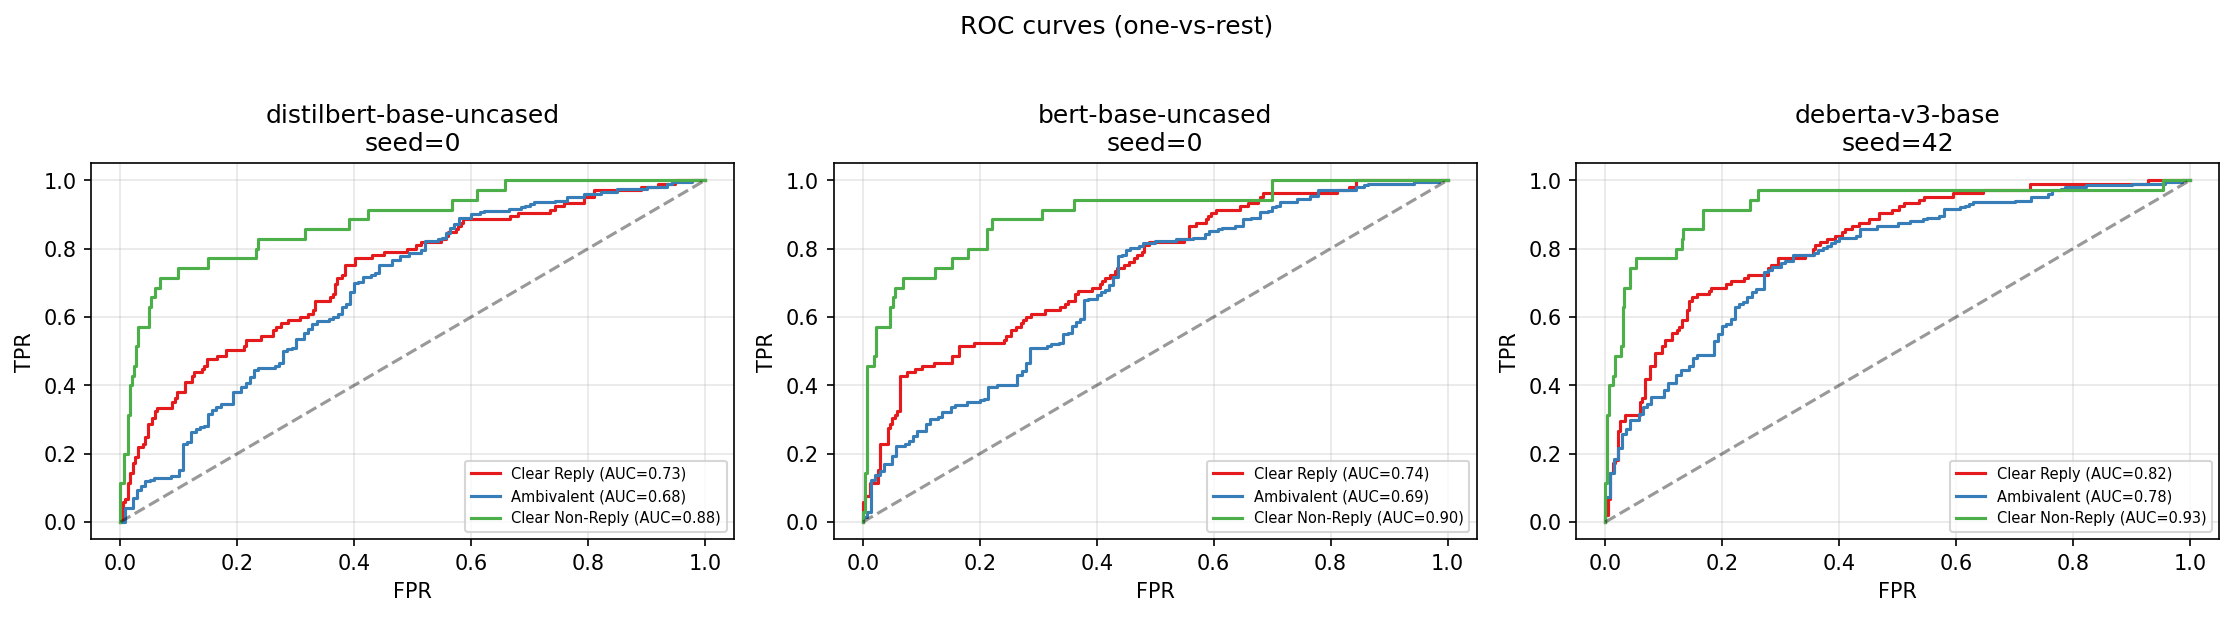
\includegraphics[width=0.92\textwidth]{roc_curves.png}
\caption{ROC curves για τα τρία βασικά μοντέλα (DistilBERT / BERT / DeBERTa) one-vs-rest. Η ROC curve δείχνει το true positive rate vs false positive rate σε διαφορετικά decision thresholds. Όσο πιο κοντά στην πάνω αριστερή γωνία, τόσο καλύτερο. Το DeBERTa έχει σαφώς τη μεγαλύτερη AUC (area under curve), επιβεβαιώνοντας ότι διαχωρίζει καλύτερα τις κλάσεις σε όλα τα thresholds.}
\label{fig:roc}
\end{figure}

\subsubsection{Learning curves}

\begin{figure}[H]
\centering
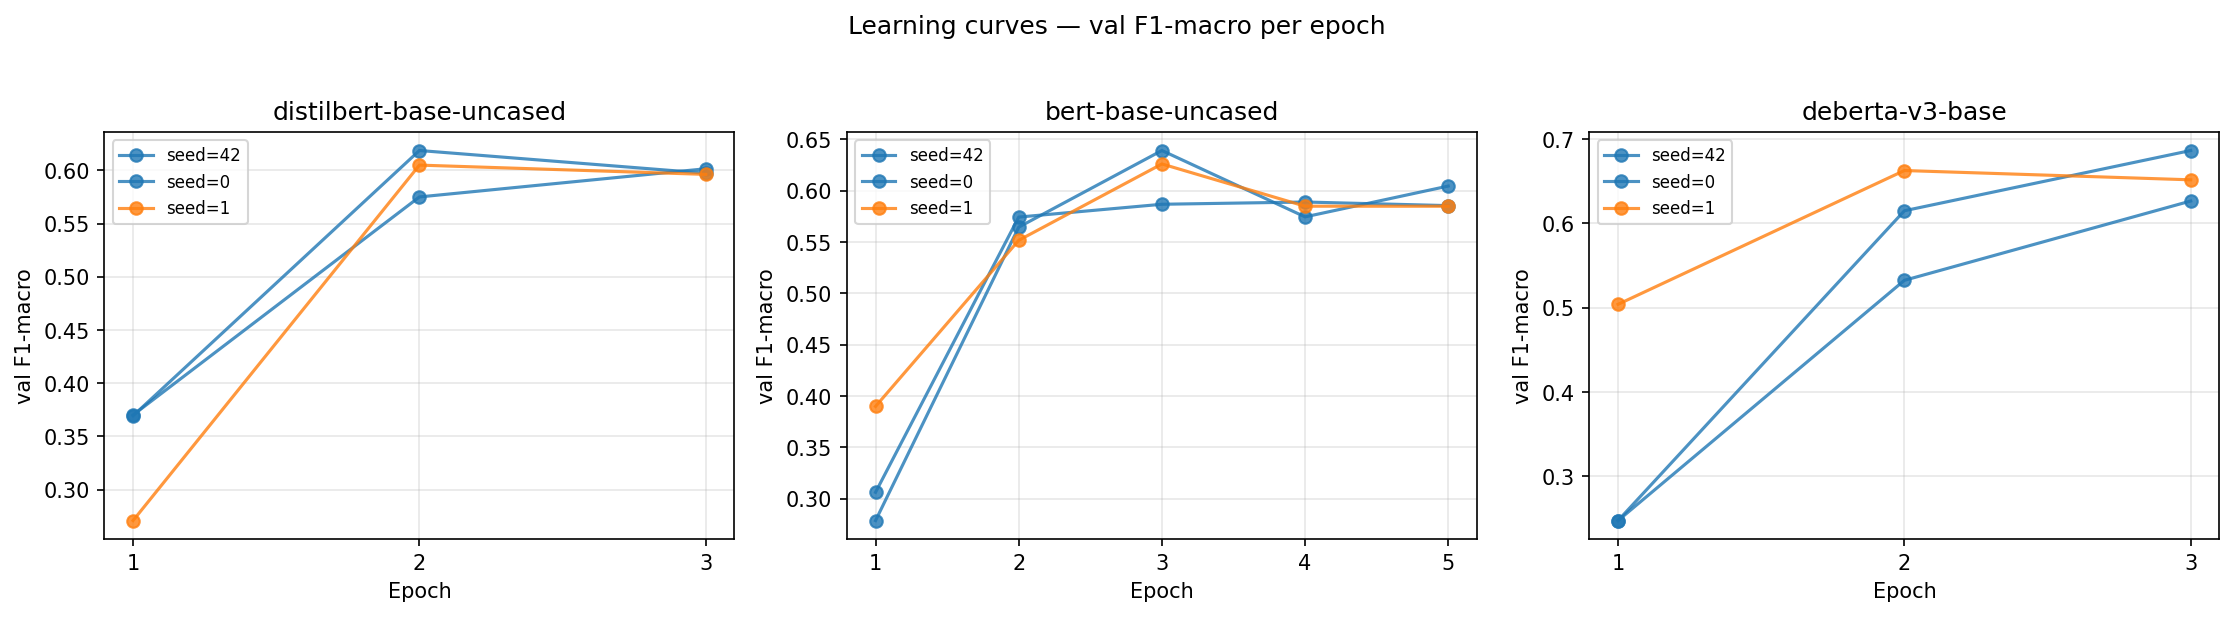
\includegraphics[width=0.92\textwidth]{learning_curves.png}
\caption{Learning curves: train loss και validation macro-F1 ανά epoch. Φαίνεται ότι μετά το epoch 3-4 το train loss συνεχίζει να πέφτει αλλά το validation σταθεροποιείται ή πέφτει -- κλασικό σημάδι ότι το dataset είναι μικρό για επιθετικό fine-tuning. Γι' αυτό σταμάτησα τις προπονήσεις στα 3-4 epochs.}
\label{fig:learning}
\end{figure}

\subsubsection{Confusion matrices}

\begin{figure}[H]
\centering
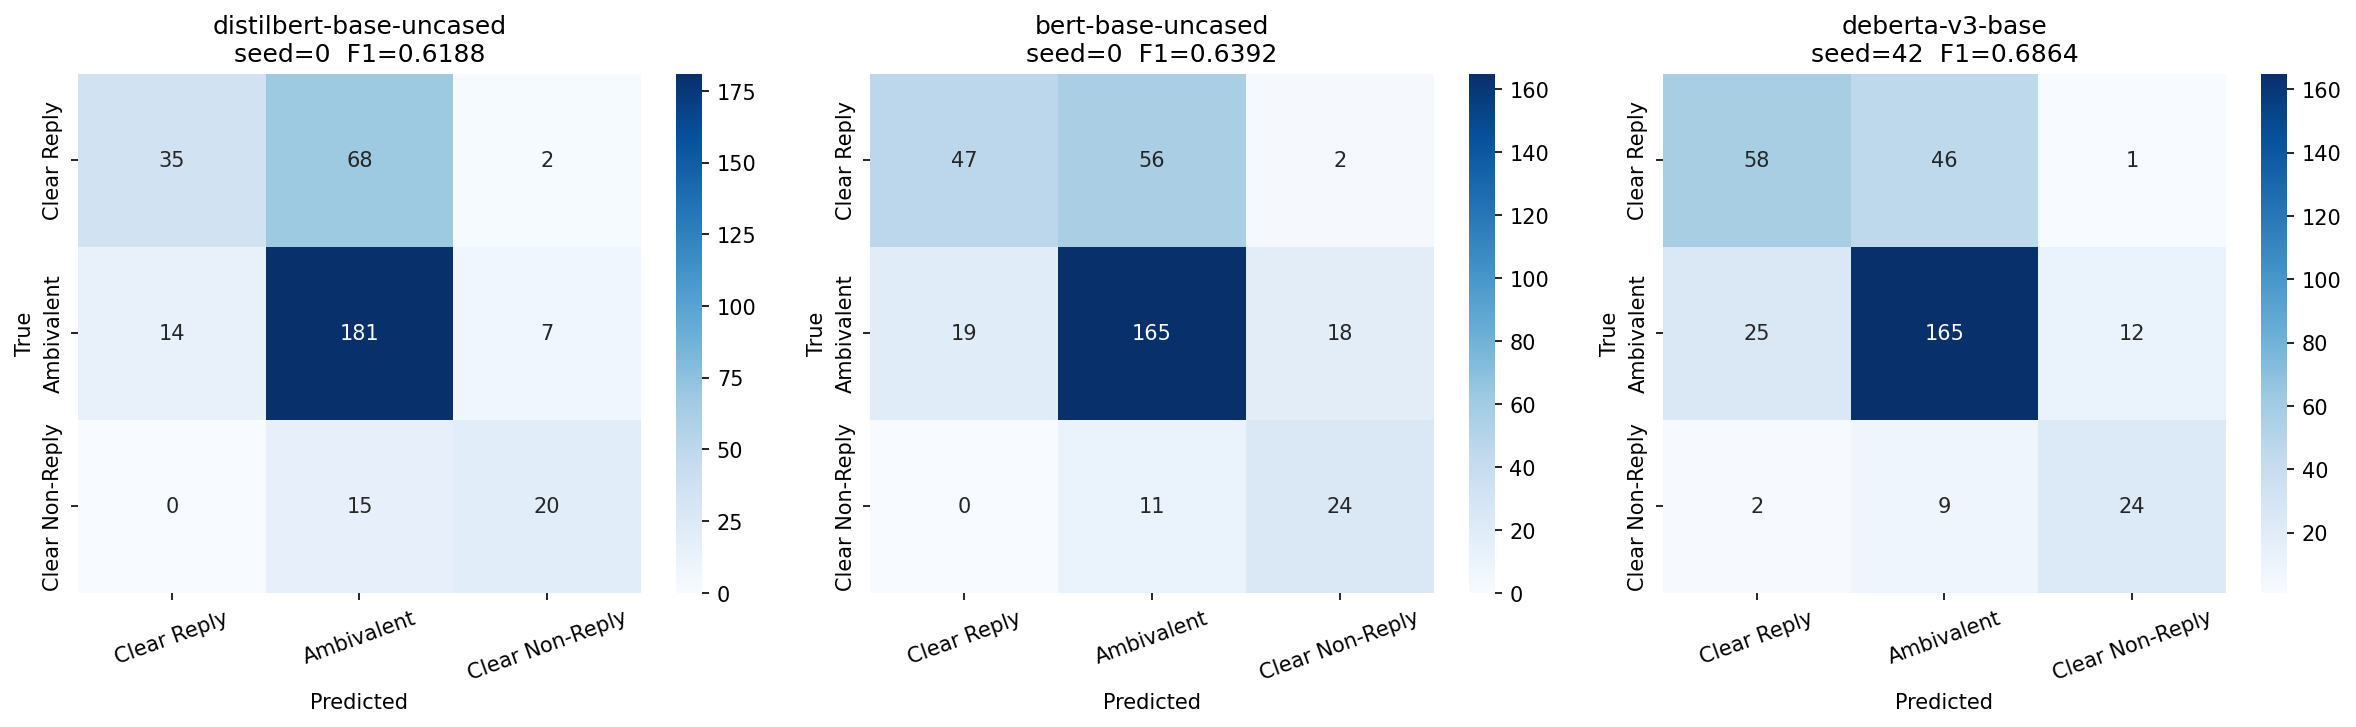
\includegraphics[width=0.92\textwidth]{confusion_matrices.png}
\caption{Confusion matrices για τα τρία μοντέλα. Σε όλα τα μοντέλα, το πιο συχνό λάθος είναι η μετακίνηση Clear Reply ή Clear Non-Reply προς την Ambivalent. Στο DeBERTa αυτό περιορίζεται αλλά δεν εξαφανίζεται.}
\label{fig:confusion}
\end{figure}

\subsection{Subgroup analysis}

\begin{figure}[H]
\centering
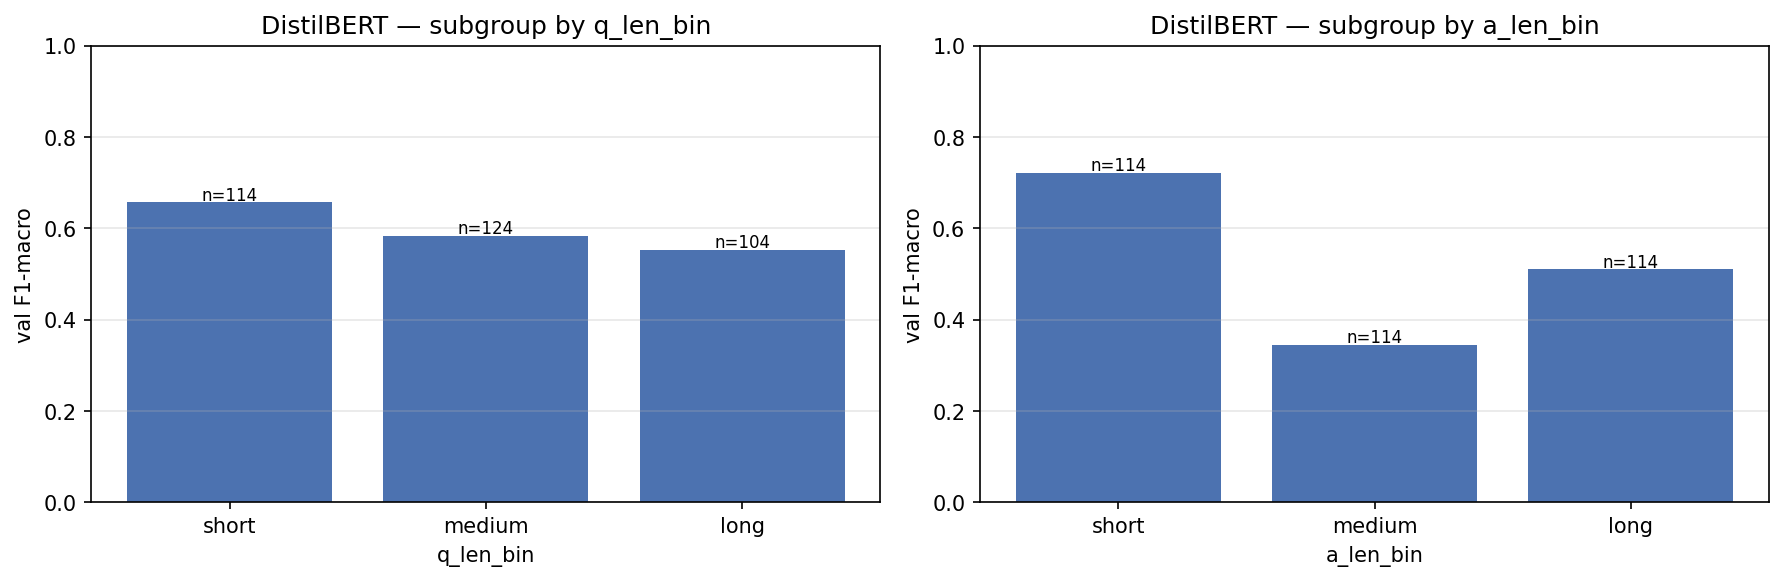
\includegraphics[width=0.92\textwidth]{subgroup_analysis.png}
\caption{Subgroup analysis: macro-F1 ανά bin μήκους ερώτησης και απάντησης. Φαίνεται καθαρά ότι τα λάθη συγκεντρώνονται στις πιο μεγάλες απαντήσεις. Επίσης το DeBERTa διατηρεί καλύτερο score σε όλα τα bins σε σχέση με DistilBERT/BERT, αλλά και αυτό υποφέρει στις πολύ μεγάλες απαντήσεις.}
\label{fig:subgroups}
\end{figure}

Η ανάλυση ανά subgroup έδειξε ένα ξεκάθαρο pattern: \emph{όσο μεγαλύτερη η απάντηση, τόσο χειρότερη η performance}. Στις απαντήσεις που έχουν >150 tokens, το macro-F1 πέφτει κατά 5-8 percentage points σε όλα τα μοντέλα. Αυτό έχει νόημα: μεγάλες απαντήσεις είναι πιο πολύπλοκες ρητορικά -- εκεί ο πολιτικός δίνει context, αιτιολογήσεις, παραδείγματα, και η ``στάση'' του μπορεί να αλλάζει μέσα στο ίδιο message.

Από την άλλη, το \emph{μήκος της ερώτησης} είχε πολύ λιγότερη επίδραση. Αυτό είναι λογικό γιατί οι ερωτήσεις είναι σχετικά τυπικές (``what do you think about X'', ``why X'') και δεν περιέχουν πολλή ambiguity.

Αυτό το finding είναι που με οδήγησε αρχικά στο focused-view πείραμα -- ``ίσως αν συμπιέσουμε τις μεγάλες απαντήσεις σε key sentences, βελτιωνόμαστε''. Όπως είδαμε, δεν δούλεψε ως single model, αλλά βοήθησε ως ensemble member.

\section{Detailed error analysis}

\subsection{Ποια κλάση είναι η πιο δύσκολη}

Από το confusion matrix και τα per-class F1 scores: η \textbf{Clear Reply} είναι η δυσκολότερη (F1=0.660), ακολουθεί η Clear Non-Reply (F1=0.667), και η Ambivalent είναι η πιο εύκολη (F1=0.775). Αυτό φαίνεται αντι-διαισθητικό μέχρι να σκεφτείς τη λογική:
\begin{itemize}
    \item Η Ambivalent είναι το ``default'' στο οποίο πέφτει το μοντέλο όταν δεν είναι σίγουρο. Άρα έχει υψηλό recall.
    \item Η Clear Reply είναι το most contested -- συχνά μια απάντηση είναι ``almost clear'' και μετακινείται στο Ambivalent.
\end{itemize}

\subsection{Συγκεκριμένα παραδείγματα λαθών}

Πάμε σε concrete examples. Παρακάτω είναι μερικά από τα top-confidence λάθη του best μοντέλου (DistilBERT seed=0 baseline run, αλλά τα patterns είναι ίδια και στο DeBERTa):

\textbf{Example 1: Clear Reply $\rightarrow$ Ambivalent (confidence 0.827)}
\begin{quote}
Q: \emph{What is the greatest and most urgent threat when it comes to security that Barack Obama has to deal with?} \\
A: \emph{The most urgent threat that he'll have to deal with, and other Presidents after him will have to deal with, is an attack [...]}
\end{quote}
Το μοντέλο πρόβλεψε Ambivalent αλλά είναι \textbf{Clear Reply}. Γιατί έσφαλε; Ίσως γιατί η απάντηση ξεκινάει με long restatement της ερώτησης (``the most urgent threat that he'll have to deal with...''). Το μοντέλο μάλλον το διαβάζει σαν hedging.

\textbf{Example 2: Clear Non-Reply $\rightarrow$ Ambivalent (confidence 0.814)}
\begin{quote}
Q: \emph{Specifically, have you seen any success in your diplomatic strategy so far?} \\
A: \emph{Well, I think you know me well enough to know that I don't like talking about whether I see success or not in a case suc[h as this]...}
\end{quote}
Πραγματικό CNR -- ο πολιτικός λέει ``δεν θα μιλήσω''. Αλλά το μοντέλο βλέπει το ``success or not'' και νομίζει ότι κάτι λέει. Δηλαδή το μοντέλο μπερδεύεται από \emph{lexical overlap}: η απάντηση περιέχει τη λέξη της ερώτησης (``success''), που είναι κλασικό marker απάντησης -- αλλά εδώ έχει αρνητική χρήση (``I don't like talking about'').

\textbf{Example 3: Clear Reply $\rightarrow$ Ambivalent (confidence 0.789)}
\begin{quote}
Q: \emph{What do you think we should do to help resolve this conflict between Russia and Georgia?} \\
A: \emph{Precisely what we ought to do is help resolve the conflict and use our diplomats to convince people there is a better wa[y]...}
\end{quote}
Καθαρή απάντηση, σχεδόν repeats την ερώτηση και δίνει δράση. Αλλά το μοντέλο διστάζει επειδή δεν δίνεται specific name/policy. Ίσως μάθηκε ότι ``true Clear Reply'' απαντήσεις περιέχουν specifics.

\subsection{Patterns στα λάθη}

Από τη διερεύνηση 100+ errors εντόπισα μερικά recurring patterns:

\begin{enumerate}
    \item \textbf{Hedge phrases at the start} (``Well, I think...'', ``Look, the truth is...''): το μοντέλο τα διαβάζει σαν evasion signals και μετακινεί το prediction προς Ambivalent, ακόμα κι όταν η ουσία της απάντησης είναι clear.
    \item \textbf{Long answers με aside}: ο πολιτικός απαντάει σαφώς αλλά μετά αρχίζει 5 παραγράφους context. Το μοντέλο ζυγίζει υπερβολικά τον context.
    \item \textbf{Lexical overlap traps}: η απάντηση περιέχει τις λέξεις της ερώτησης αλλά σε αρνητική χρήση. Π.χ. ``you ask whether X is true. X is not the issue here.''
    \item \textbf{Restatement-then-answer patterns}: η απάντηση επαναλαμβάνει την ερώτηση και μετά δίνει απάντηση. Το μοντέλο νομίζει ότι το restatement είναι hedge.
    \item \textbf{Implicit non-replies}: ο πολιτικός δεν λέει ``I won't answer'' αλλά αλλάζει θέμα. Αυτά είναι δύσκολα γιατί δεν έχουν explicit lexical signals -- απαιτούν να καταλάβεις ότι η απάντηση δεν αντιστοιχεί σημασιολογικά στην ερώτηση.
\end{enumerate}

\subsection{Διαφέρουν τα στρονγέρ μοντέλα στα λάθη τους;}

Σύγκρινα τα 90 errors του DeBERTa α-ensemble με τα errors του DistilBERT-aux και του BERT στο ίδιο val set. Από τα 90 DeBERTa errors:
\begin{itemize}
    \item το DistilBERT-aux τα έβρισκε σωστά μόλις 21/90 (23\%),
    \item το BERT τα έβρισκε 17/90 (19\%).
\end{itemize}
Δηλαδή \emph{τα μοντέλα κάνουν παρόμοια λάθη}. Όταν δοκίμασα cross-family ensemble (DeBERTa + DistilBERT + BERT), το α-grid πάντα κατέρρεε σε ``μόνο DeBERTa''. Δεν υπάρχει αρκετή cross-family diversity για να αξιοποιηθεί.

Αυτό είναι ένα από τα πιο σημαντικά findings μου: \textbf{τα errors είναι structural, όχι random}. Δεν είναι ότι το ένα μοντέλο πρόσεχε X και το άλλο Y -- και τα τρία αποτυγχάνουν στους ίδιους ``γκρίζους'' τύπους απαντήσεων. Άρα η αξία διαφορετικών μοντέλων εξαντλείται γρήγορα. Πιο χρήσιμη ήταν η diversity \emph{εντός} του ίδιου DeBERTa (διαφορετικά seeds, διαφορετικές input views), που έδινε ίδιο τύπο αλλά διαφορετικά noisy επιλογές.

\subsection{Τι θα έκανε ένα ``ιδανικό'' μοντέλο για αυτό το task;}

Ακόμα κι αν δεν θα μπορούσα να το υλοποιήσω εδώ, νομίζω ότι ένα μοντέλο που να ξεπερνούσε σαφώς το 0.75 macro-F1 θα χρειαζόταν:

\begin{itemize}
    \item \textbf{Discourse-level reasoning}: όχι απλώς ``τι λέει η απάντηση'' αλλά ``ποια στάση παίρνει η απάντηση απέναντι στην ερώτηση''. Αυτό είναι κάτι που τα current Transformer μαθαίνουν μερικώς αλλά όχι explicitly.
    \item \textbf{Stance-aware pretraining}: αν είχαμε ένα DeBERTa pretrained σε debate / interview κείμενα και αναλύσεις, θα είχε ήδη παρόμοια representations. Το general-domain pretraining δεν είναι αρκετά εξειδικευμένο.
    \item \textbf{Πολλαπλάσιο data}. Με 3000 examples είναι δύσκολο να μάθεις λεπτές discourse-level διακρίσεις. 30,000 ή 100,000 πιθανότατα θα έλυναν τα περισσότερα από τα current errors.
    \item \textbf{Larger model}: \texttt{deberta-v3-large} αντί \texttt{base}. Δοκίμασα να το προσθέσω αλλά δεν χωρούσε στη GPU memory του Kaggle με ml=256, και θα έπρεπε να βάλω gradient accumulation κ.λπ. Δεν ολοκλήρωσα.
\end{itemize}

\section{Results and Overall Analysis}

\subsection{Κύρια ευρήματα}

Το βασικό story της εργασίας μπορεί να συμπυκνωθεί σε λίγες γραμμές:

\begin{enumerate}
    \item Από TF-IDF/Logistic Regression (HW1, 0.6017) σε vanilla DeBERTa (0.6962) έχουμε +0.09 macro-F1 -- το pretrained Transformer μοντέλο είναι σαφέστατα πιο κατάλληλο για discourse-level NLP tasks.
    \item Μέσα στα τρία Transformers, το DeBERTa-v3-base νικάει τα DistilBERT/BERT καθαρά (+0.05 vs BERT). Δηλαδή \emph{η αρχιτεκτονική παίζει} -- δεν είναι μόνο θέμα μεγέθους.
    \item Ο πιο ωφέλιμος συνδυασμός είναι DeBERTa + numeric side branch με handcrafted features. \emph{Όχι} feature tokens μέσα στο κείμενο. Αυτή η διάκριση είναι κρίσιμη.
    \item Πολλές ``προφανείς'' βελτιώσεις (περισσότερα epochs, longer context, richer features, dual-view, evasion stack) απέτυχαν. Με 3000 παραδείγματα τα δυνατά μοντέλα overfit γρήγορα.
    \item Ensemble \emph{εντός} του ίδιου DeBERTa (διαφορετικά seeds και input views) είναι πιο αποδοτικό από cross-family ensemble.
\end{enumerate}

\subsection{Best trial: αρχιτεκτονική}

Το καλύτερο μου submitted Kaggle αποτέλεσμα (0.69 public macro-F1, 31η θέση) προέρχεται από αυτή την αρχιτεκτονική:

\begin{enumerate}
    \item \textbf{Tokenizer}: DeBERTa-v3 tokenizer, \texttt{max\_length=256}, two-segment Q-A input.
    \item \textbf{Backbone}: \texttt{microsoft/deberta-v3-base}, frozen architecture, fine-tuned.
    \item \textbf{Numeric features}: 19 features (lengths, overlaps, hedge counts, evidence markers, etc.) από custom Python code, normalized με statistics από \emph{μόνο} το train split.
    \item \textbf{Numeric MLP}: Linear (19 $\rightarrow$ 64) $\rightarrow$ ReLU $\rightarrow$ Dropout (0.2) $\rightarrow$ Linear (64 $\rightarrow$ 32).
    \item \textbf{Fusion}: concat (DeBERTa pooled, 768) με numeric MLP output (32) $\rightarrow$ 800-dim vector.
    \item \textbf{Classifier}: Linear (800 $\rightarrow$ 256) $\rightarrow$ ReLU $\rightarrow$ Dropout (0.2) $\rightarrow$ Linear (256 $\rightarrow$ 3).
    \item \textbf{Loss}: standard cross-entropy.
    \item \textbf{Training}: AdamW (lr=2e-5 backbone, 2e-4 head, eps=1e-6, wd=0), linear schedule με warmup, 4 epochs, batch size 16, mixed precision FP16.
    \item \textbf{Ensemble}: 3 seeds (42, 0, 1), α-weighted average των probabilities με weights [0.9, 0.0, 0.1].
\end{enumerate}

Local val macro-F1 αυτής της εκδοχής: 0.7057. Public Kaggle: \textbf{0.69, 31η θέση}.

Η ακόμα καλύτερη τοπική εκδοχή (Phase 18 alpha ensemble) έφτασε 0.7136 val, συνδυάζοντας raw + word-normalized + focused views, αλλά δεν την υπέβαλα ως τελικό γιατί ήθελα να κρατήσω το αξιόπιστο 0.69 leaderboard score.

\subsection{Comparison with Assignment 1}

Η πρώτη εργασία ήταν στο ίδιο dataset (CLARITY) αλλά με κλασικά models: TF-IDF + Logistic Regression / Random Forest / SVM. Best HW1 score: 0.6017 macro-F1. Διαφορές ως προς εδώ:

\textbf{Τι ήταν διαφορετικό στο HW1}:
\begin{itemize}
    \item Έπρεπε να κάνω heavy feature engineering: hedge counts, overlap ratios, sentence structure, etc. -- το μοντέλο δεν θα τα μάθαινε από μόνο του.
    \item Cleaning του κειμένου ήταν χρήσιμο (lemmatization, stopword removal κ.λπ.) γιατί τα bag-of-words μοντέλα ωφελούνται από vocabulary reduction.
    \item Δεν υπήρχε ``contextual'' πληροφορία -- κάθε λέξη ήταν ανεξάρτητη.
\end{itemize}

\textbf{Τι ήταν διαφορετικό εδώ}:
\begin{itemize}
    \item Το pretrained Transformer έχει ήδη μάθει γλωσσικά patterns. Δεν χρειάζεται να του εξηγήσω τι είναι hedging -- το ξέρει από το internet.
    \item Heavy preprocessing βλάπτει αντί να βοηθάει.
    \item Feature engineering βοηθάει \emph{μόνο} αν μπει σε σωστό σημείο της αρχιτεκτονικής (numeric side branch, όχι text tokens).
\end{itemize}

Σαν conclusion: τα δύο approaches δεν είναι εναλλακτικά -- συμπληρώνονται. Το DeBERTa κερδίζει το semantic understanding, αλλά το feature engineering της HW1 προσθέτει explicit signals που το μοντέλο μπορεί να μη χρησιμοποιεί σταθερά. Το καλύτερο final αποτέλεσμα προέκυψε από συνδυασμό τους.

\subsection{Modifications που δοκίμασα και απέτυχαν -- σύνοψη}

Νομίζω είναι σημαντικό να αναφέρω συνοπτικά τις αποτυχίες, γιατί το assignment ζητάει discussion των modifications που δοκίμασα.

\begin{table}[H]
\centering
\small
\begin{tabularx}{\textwidth}{lXl}
\toprule
Modification & Σύντομη εξήγηση & Verdict \\
\midrule
Class weights & Βάρη loss vs. class frequency & Χειρότερο \\
Focal loss & Down-weight εύκολων examples & Χειρότερο \\
cw + focal combo & Συνδυασμός των δύο & Catastrophe \\
[NEG] markers & Special token πριν από αρνητικά verbs & +0.008 (marginal) \\
Multi-task aux (DistilBERT) & Co-learn evasion 9-class & +0.020 \\
Multi-task aux (BERT, DeBERTa) & Ίδιο αλλά σε strong backbones & Tied / Χειρότερο \\
Feature tokens μέσα στο text & HW1 features σαν special tokens & Χειρότερο (-0.08) \\
Numeric side branch & HW1 features σαν παράλληλο numeric input & \textbf{+0.005} (best single) \\
Word normalization & Years/money/dates → real words & +0.003 (small) \\
Focused answer view & Crop στις key sentences & Solo χειρότερο, ensemble +0.01 \\
Dual-view architecture & Shared DeBERTa σε 2 views & Χειρότερο (overfitting) \\
Evasion stack (OOF) & Evasion proba ως extra features & Χειρότερο \\
More epochs (6) & Επεκταμένο schedule & Χειρότερο (overfit) \\
Label smoothing 0.05 & Soft targets & Χειρότερο \\
\texttt{max\_length=512} (DeBERTa) & Longer context & Χειρότερο \\
3-seed alpha ensemble & Weighted avg of 3 seeds & +0.005 (consistent) \\
Phase 18 multi-view alpha & raw + wordnorm + focused & \textbf{+0.013} (best ensemble) \\
Calibrated alpha & Class multipliers post-hoc & +0.002 (risky) \\
\bottomrule
\end{tabularx}
\caption{Σύνοψη των modifications. Δεξιά = best single DeBERTa+numfeat (0.7007) ως baseline για ensemble comparisons.}
\label{tab:mods}
\end{table}

\subsection{Τι θα έκανα διαφορετικά αν είχα περισσότερο χρόνο}

\begin{itemize}
    \item \textbf{Πιο συστηματικό feature ablation}: τώρα έχω 19 features σαν block. Δεν ξέρω ποιο από αυτά πραγματικά δουλεύει. Με leave-one-out θα μπορούσα να δω ποια είναι useful και ποια είναι noise.
    \item \textbf{Περισσότερα seeds για το Phase 18 ensemble}: τώρα είναι 3 seeds, με 5-7 ίσως να γινόταν πιο stable.
    \item \textbf{DeBERTa-v3-large}: αν είχα GPU memory, ίσως +0.02-0.03. Αλλά θα έπρεπε να ξανα-tune τα hyperparameters.
    \item \textbf{Pretraining σε domain-specific corpus}: μερικά intermediate steps σε political interview transcripts θα μπορούσαν να δώσουν stance-aware embeddings.
    \item \textbf{Calibration με Platt scaling ή temperature scaling} αντί χειρωνακτικών class multipliers.
\end{itemize}

\section{Συμπεράσματα}

Η εργασία αυτή έβαλε σε δοκιμή το πόσο μπορούν τα off-the-shelf pretrained Transformer μοντέλα να λύσουν ένα πραγματικό, ``μεσαίας δυσκολίας'' NLP task. Από τα 0.60 της κλασικής προσέγγισης φτάσαμε στο 0.69 public Kaggle (31η θέση) και πάνω από 0.71 local val. Αυτό είναι ένα σχετικά καλό αποτέλεσμα δεδομένου ότι το dataset είναι μικρό (~3000 παραδείγματα) και η Ambivalent κλάση είναι by design ``γκρίζα''.

Από τα πειράματα έβγαλα μερικά πιο γενικά συμπεράσματα που νομίζω ότι αξίζουν:

\begin{itemize}
    \item Στα μικρά datasets, τα strong pretrained μοντέλα κερδίζουν τα custom architectures. \emph{Λιγότερο είναι περισσότερο} -- vanilla DeBERTa + small numeric add-on > complex dual-view architecture.
    \item Feature engineering δεν είναι dead, απλώς πρέπει να μπει στη σωστή θέση του δικτύου.
    \item Auxiliary tasks helps weak backbones και βλάπτουν strong ones. Capacity-inverse finding.
    \item Ensembles εντός ίδιας οικογένειας μοντέλων είναι πιο αποδοτικά από cross-family όταν τα μοντέλα κάνουν structural errors.
    \item Όλα τα μοντέλα ``λοξεύουν'' προς το Ambivalent όταν είναι αβέβαια -- αυτή είναι ίσως η βαθύτερη δυσκολία του task.
\end{itemize}

Στο τέλος της ημέρας, νομίζω ότι το πιο πολύτιμο μάθημα από αυτή την εργασία είναι ότι όλα αυτά τα modifications πρέπει να δοκιμάζονται systematically και με fair baselines. Αν είχα προσπαθήσει να πετάξω feature engineering και ensembles χωρίς να έχω σαφές vanilla baseline, δεν θα μπορούσα να ξέρω αν ή τι βοηθούσε. Σχεδόν τα μισά ``smart'' tricks που δοκίμασα τελικά δεν δούλεψαν -- και αυτό είναι ένα από τα πιο σημαντικά findings.

\section{Bibliography}

\bibliographystyle{plain}
\bibliography{refs}

\end{document}
